\section{Thrust 2. LLM-based Intelligent Test Case Generation}
\label{sec:thrust2}

%------------------- TEST CASE GENERATION PROMPTS FIGURE --------------------



%\subsection{The Test Case Generation Module}

\begin{wrapfigure}{l}{0.53\textwidth}
  \centering
	\lstset{
		numbers=left,
		numberstyle= \tiny,
		keywordstyle= \color{blue!70},
		commentstyle= \color{red!50!green!50!blue!50},
		frame=shadowbox,
		rulesepcolor= \color{red!20!green!20!blue!20} ,
		xleftmargin=1.5em,xrightmargin=0em, aboveskip=1em,
		framexleftmargin=1.5em,
                numbersep= 5pt,
		language=Java,
    basicstyle=\scriptsize\ttfamily,
    numberstyle=\scriptsize\ttfamily,
    emphstyle=\bfseries,
                moredelim=**[is][\color{red}]{@}{@},
		escapeinside= {(*@}{@*)}
	}
%\begin{minipage}{.48\textwidth}        
\begin{lstlisting}[caption = ]
(*@{\color{orange}{PROMPT} Coverage Increasing Test Case Generation@*)
Generate a single test case for a Java program to cover uncovered lines of code denoted by '!'. Provide only the test input without explanations. Consider various conditions, edge cases, and typical use cases.
The test case input is in the following:
Test Case Input:
<input 1>
<input 2>...
\end{lstlisting}
%\end{minipage}
\vspace{-6pt}
\caption{Prompt to generate test cases intended to increase coverage}
\label{fig:cov-prompt}
\end{wrapfigure}


This section presents the design of the interactions via prompting
between the LLMs used for test case generation.
%These prompting steps correspond to the two API calls to the LLM at
%line 7 and line 9 of Listing~\ref{algo}, and the call to coverage
%prediction LLM in CodePilot~\cite{forge24} at line 10 if
%Listing~\ref{algo}.
The Test Case Generation module, operated by prompting GPT, is
responsible for creating test mutations based on the coverage achieved
by the current test suite. Within {\tool}, we utilize a parameter
denoted as $N$, representing the number of test mutations
%(lines 7 and 9, Listing~\ref{algo})
that will be generated alongside the test seed $T\_seed$. Within the
test case generation loop,
%(line 5, Listing~\ref{algo}),
we implement two distinct strategies, each corresponding to a
different prompt and purpose. One strategy is devised to generate test
cases targeting various vulnerable areas, while the other strategy
focuses on each area individually to identify runtime
errors/exceptions.

\subsubsection*{Prompting for Coverage Increasing Test Case Generation}

As {\tool} functions as a coverage-guided fuzzing framework, increasing coverage stands as a primary objective. Consequently, if the cumulative coverage of the existing test suite hasn't yet achieved 100\%, and the generated test cases did not contribute towards reaching higher cumulative coverage, the immediate focus shifts to increasing code coverage in the subsequent cycle. This prompt responsible for Test Case Generation is directed to create test cases likely to extend coverage by targeting the portions of code that remain uncovered. (prompt depicted in Fig.~\ref{fig:cov-prompt}).





\begin{wrapfigure}{l}{0.53\textwidth}
	\lstset{
		numbers=left,
		numberstyle= \tiny,
		keywordstyle= \color{blue!70},
		commentstyle= \color{red!50!green!50!blue!50},
		frame=shadowbox,
		rulesepcolor= \color{red!20!green!20!blue!20} ,
		xleftmargin=1.5em,xrightmargin=0em, aboveskip=1em,
		framexleftmargin=1.5em,
                numbersep= 5pt,
		language=Java,
    basicstyle=\scriptsize\ttfamily,
    numberstyle=\scriptsize\ttfamily,
    emphstyle=\bfseries,
                moredelim=**[is][\color{red}]{@}{@},
		escapeinside= {(*@}{@*)}
	}
\hspace{8pt}
%\begin{minipage}{.4\textwidth}        
\begin{lstlisting}[caption = ]
(*@{\color{orange}{PROMPT} Runtime-error-detection Test Case Generation@*)
Generate a single test case without providing an explanation for to raise the following scenarios in a Java program:

InputMismatchException: Provide an input value that whose data type is different than the one specified. 
ArithmeticException: Test cases that could raise arithmetic exceptions include division by zero, overflow, underflow, and attempts to perform invalid operations such as taking the square root of a negative number.
NullPointerException: Create a scenario where a variable is explicitly set to null before usage.
NumberFormatException: Input a value that cannot be parsed to the expected data type (e.g., a non-numeric string).
ArrayIndexOutOfBoundsException or IndexOutOfBoundsException: Design input values that lead to accessing array or list indices beyond their bounds.
(Other types of runtime errors and exceptions)
Ensure the test case input is in the following:
Test Case Input:
<input 1>
<input 2>...
Generate a single test case without providing an explanation for the below Java program:
\end{lstlisting}
%\end{minipage}
\vspace{-12pt}
\caption{Prompt to generate test cases intended to catch errors}
\label{fig:exception-prompt}
\end{wrapfigure}

The sole purpose of the prompt is to produce a test case that
comprehensively covers lines of code not previously traversed by test
cases in the current suite. In the prompt, the LLM receives the code
coverage information of the current test suite, denoted by `$>$' and
`!' for covered and uncovered lines, respectively. We
also instruct the LLM to produce the output in a specific format,
where different scenarios are considered, such as negative,
positive, zero inputs, and maximum values, thus reflecting a
diverse range of inputs.

\subsubsection*{Prompting for Runtime-Exception-Detection Test Case Generation}

Once the target of achieving 100\% coverage is met or a test case
effectively covers previously unexplored code segments, the focus
shifts towards uncovering potential runtime exceptions.
%
This strategy is designed to prompt the LLM towards generating test
cases aimed at capturing runtime errors and
exceptions. Fig.~\ref{fig:exception-prompt} illustrates the structures
and intricacies of our prompt for this strategy. The initial segment
is dedicated to predicting and providing insights into various
potential unhandled runtime exceptions. The objective is to generate
test cases to explore diverse facets of runtime exceptions
comprehensively. We also instruct the LLM to output in a specific
format. We expect that this strategy complements the
coverage-increasing test case generating prompt to efficiently produce
high-quality test cases, thus delivering a thorough assessment of the
target program.

\subsubsection*{Preliminary Experimental Results on Runtime Error Detection}
\label{sec:rq1}

%\subsection{Baseline and Procedure}

{\bf Baselines and Metrics.} In this study, we chose Jazzer~\cite{jazzer}, an
open-source fuzz testing tool for Java due to its popularity and
availability.
%
Both coverage-guided fuzzing approaches were configured to operate
continuously for a duration of 5 minutes. For Jazzer, this limit
period encompasses the fuzzing process, which involves test case
generation, execution for coverage and bug detection, and the
integration of pertinent test mutations into the corpus for subsequent
testing iterations. Notably, the timeout duration excludes the build
and compilation phases to ensure fair comparison.  Conversely, for
{\tool}, the 5-minute limit encompasses all the steps within the
framework, that are
integral to its coverage-guided fuzzing workflow. Upon
reaching the time limit, the execution logs of both fuzzers are
scrutinized to gather metrics essential for evaluating their
respective performances.

%\subsection{Evaluation Metrics}

\begin{wrapfigure}{l}{0.53\textwidth}
\begin{center}
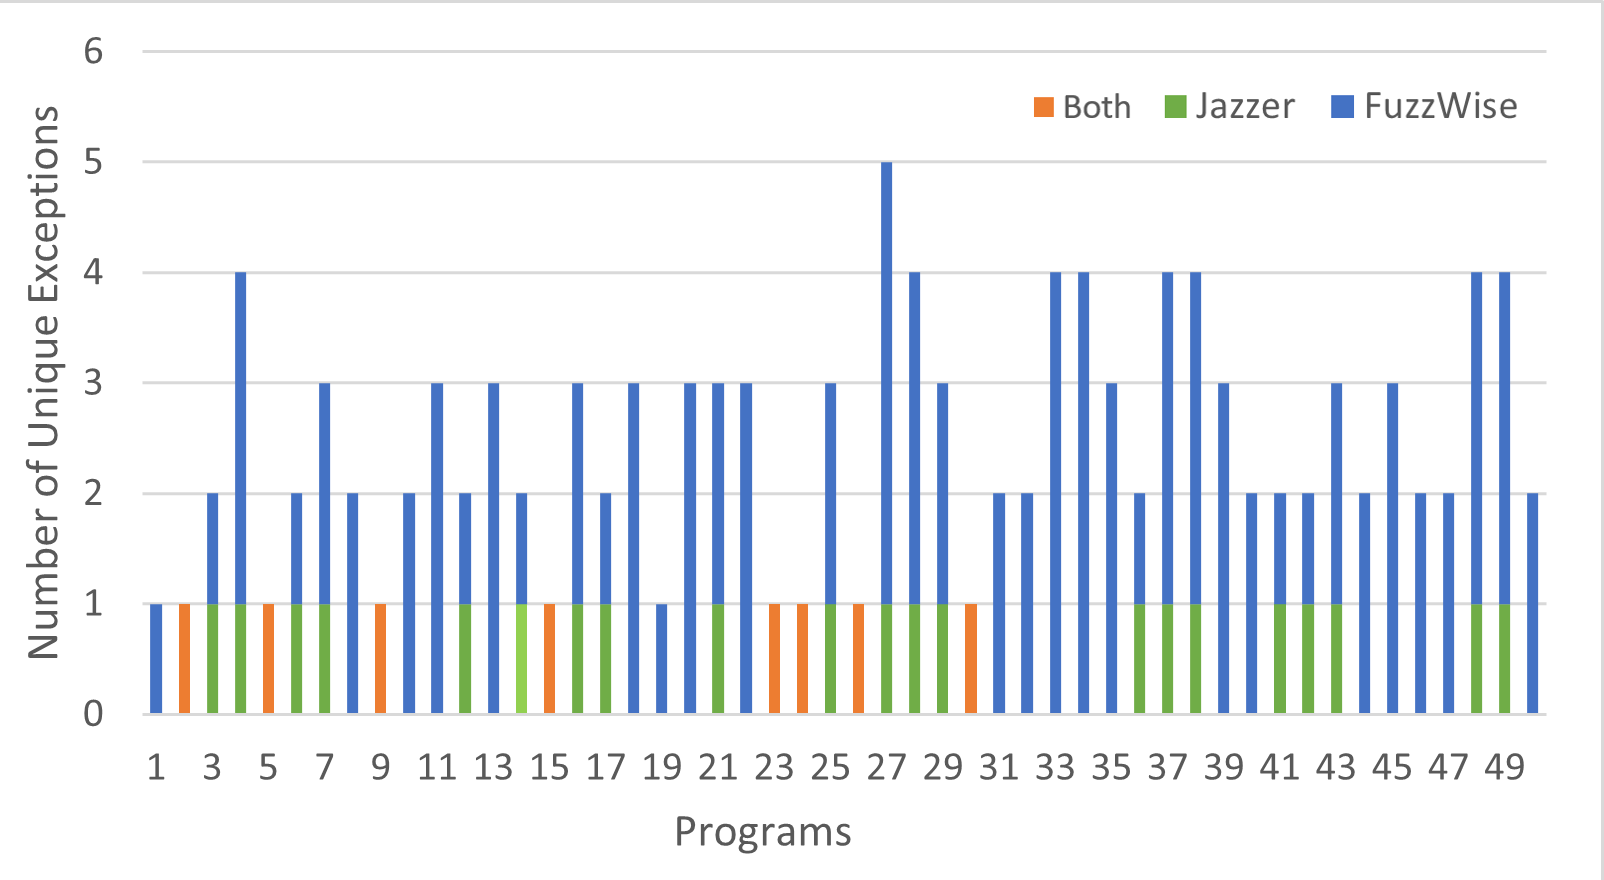
\includegraphics[width=3.5in]{RQ1a_Unique Exceptions.png}
\vspace{-21pt}
\caption{Comparative Study on Runtime Error Detection}
\label{fig:rq1-runtime-detection}
\end{center}
\end{wrapfigure}

First, we aim to measure the approaches' effectiveness in detecting
runtime errors. Within the time limit, we counted the number of unique
runtime errors/exceptions that an approach can reveal for a
program.

%This is denoted by the Number of Unique Runtime Exceptions (\code{NURE}).

Second, we also aim to measure how the test generation processes from
the approaches perform in terms of the~numbers of test cases created,
wasted, executed, and the number of effective test
cases. Thus, we use the following metrics for this study: Average
Generated Test cases (AGT), Average Executed Test cases (AXT), Average
Effective Test cases (AET), and Average Wasted Test cases (AWT). AGT
is computed as the average number of generated test cases for each
approach. AXT denotes the average number of test cases that were
actually executed on the programs to detect runtime exceptions. AET
denotes the average number of test cases that effectively detected
runtime errors. AWT signifies the average number of test cases
wasted due to their lack of influence on either coverage
improvement or bug detection. We also stratify these metrics over the
different ranges of the programs' lengths.

%It is determined as the ratio of the total number of discarded test cases by the fuzzer for all programs within a particular code length range to the number of programs within that range.

%It is computed as the ratio of the total number of executed test cases for all programs within a specified code length range to the number of programs in that range.



%In order to correctly evaluate the performance of {\tool} against Jazzer as a baseline, there are 2 crucial elements that must be compared i.e.,  the number of exceptions raised within a specified time frame, and the number of test case mutations that are not of significance to the fuzzer and are therefore, discarded. 

%To assess the performance of Jazzer and {\tool} across the dataset, we employ two types of metrics. The first type aims to evaluate performance based on the number of test cases created, executed, and discarded. Two metrics are utilized for this purpose: Average Executed Test cases (AET), and Average Discarded Test Cases (ADT).



%In summary, AET and ADT metrics provide insights into the behavior of the fuzzer concerning the execution, and discarding of test cases for programs of specific lengths. These metrics offer approximate values indicating the expected number of test cases executed, and discarded, respectively, for a given program length.

%The second type of metrics focuses on evaluating the performance of the coverage-guided fuzzers based on the number of runtime exceptions they can raise within a specified time limit. This is measured by a singular metric known as the Number of Unique Runtime Exceptions (NURE), which quantifies the unique runtime exceptions caught by the fuzzer for a single program.

%\subsection{Empirical Results}



% Figure 8 accurately depicts the NURE (Number of Unique Runtime Exceptions) values for each of 50 programs in the dataset. The maximum NURE value acheived by Jazzer (depicted im green) is 1 Exception per program wheres the maximum acheived by {\tool} is 5 exceptions in a program. It is evident that {\tool} is able to detect equal to more number of unique runtime exceptions than Jazzer for the same program within the same time frame due to the fact that {\tool} dual prompting method for test case generations.

% Additionally, When considering the number of Test Cases generated (refer to Figure 6), {\tool} generates close to 0.0065\% of the number of test cases that Jazzer generates for a program and still is successful in raising more number of unique runtime exceptions. This can be attributed to the fact that the test case mutations generated by {\tool} are more controlled and less random than Jazzer. 

% When it comes to test case execution, Jazzer executed all of the test cases that it generates, irrespective of the presence of duplicate test cases. On the other hand, {\tool} executes an average of 235 out of 315 test cases generated. This is because, before execution, {\tool} removes duplicate test cases to increase efficiency. 

% Finally, when comparing the number of test cases that both fuzzers discard due to ineffectivness or duplicacy (refer to figure 7), across a range of code length, Jazzer discards an average of 4679532 test cases for a code of length 10 to 15 lines whereas {\tool} discards an average of 305 test cases. For code of length 16-20 lines, Jazzer discards 2389922 of the test cases it generates whereas {\tool} only discards 73 of the generated test cases. For code of length  21 to 40 lines, Jazzer discards 3374709 of the test cases it generates and executes whereas {\tool} discards 23. For code length of 41 to 60 lines and 61 to 70 lines, Jazzer discards XXX(NEED TO VERIFY) and 1624254 test cases respectively whereas {\tool} discards none of the test cases it generates. {\tool} extremely low percentage of the number of test cases discarded can be attributed to the higher quality of the test case mutations generated. Since very less mutations are generated more than once, fewer have to be discarded. 

% It is also impoartant to note that as the average length of code increases, AGT, AET and AGT for both fuzzers consistently drops due to the fact that the time taken to both execute and predict the code coverage for a single test case increases with an increase in length of code.

%Fig.~\ref{fig:rq1-runtime-detection} displays the runtime error
%detection results. As seen, {\tool} is able to detect more runtime
%errors/exceptions than the baseline Jazzer. Within the time limit,
%while Jazzer can only detect at most one runtime error, {\tool} can
%detect up to 5 runtime errors. In {\bf XX} cases, Jazzer is not
%effective, while {\tool} did not detect any exception in only two
%programs.  In all 50 programs, within the time limit, {\tool} detected
%a total of {\bf XX} runtime errors, while {\tool} revealed a total of
%{\bf YY} such errors.
 
%accurately illustrates the NURE (Number of Unique Runtime Exceptions) values for each of the 50 programs within the dataset. Jazzer achieved a maximum NURE value of 1 exception per program (depicted in green), whereas {\tool} reached a maximum of 5 exceptions in a program. This indicates that {\tool} is capable of detecting a greater number of unique runtime exceptions than Jazzer for the same program within the same time frame, owing to {\tool}'s dual prompting method for test case generation.



{\bf Preliminary Results.} Fig.~\ref{fig:rq1-runtime-detection}
presents the results on runtime error detection. As seen, {\tool}
outperforms the baseline Jazzer in detecting more unique runtime
errors/exceptions. While Jazzer, within the time limit, can only
detect a maximum of one runtime error, {\tool} can identify up to 5
runtime errors. In {\bf 17} cases, Jazzer proves ineffective (no
detected error), whereas {\tool} only failed to detect any exceptions
in {\bf 3} programs. Across all 50 programs, within the given time
constraints, {\tool} successfully identified a total of {\bf 97}
runtime errors, while Jazzer only detected {\bf 26} such errors.



% \begin{figure}[t]
% \begin{center}
% \includegraphics[width=4.5in]{rq1_table.png}
% \vspace{-15pt}
% \caption{Comparison on Test Case Generation (RQ1) ({\bf FIXME} Remove ADT, add Effective Test Cases (AET), change the old AET into AXT)}
% \label{fig:rq1-agt-aet-adt-table}
% \end{center}
% \end{figure}

\begin{wraptable}{l}{0.62\textwidth}
  \centering
  \small
  \caption{Comparison on Test Case Generation}
\label{tab:rq1coverageeval}
%\renewcommand{\arraystretch}{1.2} % Adjust the vertical spacing
%\resizebox{\columnwidth}{!}{%
\begin{tabular}{c|ccc|ccc}
\hline
\multirow{2}{*}{\textbf{Length of Code (Lines)}} & \multicolumn{3}{c|}{\textbf{Jazzer}} & \multicolumn{3}{c}{\textbf{FuzzWise}} \\ \cline{2-7} 
 & \multicolumn{1}{c|}{AGT} & \multicolumn{1}{c|}{AXT} & AET & \multicolumn{1}{c|}{AGT} & \multicolumn{1}{c|}{AXT} & AET \\ \hline
10 to 15 & \multicolumn{1}{c|}{8,083,663} & \multicolumn{1}{c|}{8,083,663} & 4,009,232 & \multicolumn{1}{c|}{513} & \multicolumn{1}{c|}{251} & 181 \\
16 to 20 & \multicolumn{1}{c|}{5,040,462} & \multicolumn{1}{c|}{5,040,462} & 2,520,225 & \multicolumn{1}{c|}{249} & \multicolumn{1}{c|}{176} & 128 \\
21 to 40 & \multicolumn{1}{c|}{3,374,709} & \multicolumn{1}{c|}{3,374,709} & 1,147,240 & \multicolumn{1}{c|}{197} & \multicolumn{1}{c|}{174} & 122 \\ 
41 to 60 & \multicolumn{1}{c|}{2,918,978} & \multicolumn{1}{c|}{2,918,978} & {661,458} & \multicolumn{1}{c|}{118} & \multicolumn{1}{c|}{118} & 66 \\
61 to 70 & \multicolumn{1}{c|}{1,667,523} & \multicolumn{1}{c|}{1,667,523} & 372,470 & \multicolumn{1}{c|}{99} & \multicolumn{1}{c|}{99} & 65 \\ \hline
\end{tabular}%
%}
%\vspace{4pt}
\end{wraptable}

Table~\ref{tab:rq1coverageeval} shows the detailed results.
%on the number of generated test cases (\code{AGT}), the number of
%executed test cases (\code{AET}), and the number of discarded test
%cases (\code{ADT}).
We group them accordingly to the sizes of the programs. As seen,
regarding the number of generated test cases, {\tool} produced
significantly fewer test cases, accounting for approximately 0.0065\%
of the number of test cases generated by Jazzer for a given
program. However, despite this disparity, {\tool} successfully
identified more unique runtime exceptions.

Regarding the executed test cases, Jazzer, by design, executed all
generated test cases, including duplicates. In contrast, {\tool} {\em
  executed an average of 235 out of 315 generated test cases}. On
average, Jazzer executed {\bf 4,217,067} test cases per program, while
{\tool} executed only {\bf 235} test cases. Combined with the findings
depicted in Fig. \ref{fig:rq1-runtime-detection}, it's evident that
{\tool} is more efficient in runtime error detection compared to the
baseline: on average, {\tool} executed {\bf 1,742,125} generated test cases
to detect a runtime error, while Jazzer executed {\bf 112} test cases
per exception.

%{\bf Add a paragraph to discuss the result in the Fig. about the
%  generated test cases that are effective in bug detection. Also, add
%  the ratio between the number of effective test cases over the number
%  of generated test cases}.

%Regarding effective test cases, as seen in
%Fig.~\ref{fig:rq1-runtime-detection}, on average, {\tool} generates a
%higher number of effective test cases than Jazzer, i.e., more
%effective in error detection, {\bf XX} versus {\bf YY}. Additionally,
%the ratio between the number of effective test cases over the total
%number of generated ones for {\tool} ({\bf XX}) is also higher than that
%ratio for Jazzer ({\bf YY}). This shows that {\tool} is more efficient
%in effective test case generation.

In terms of effective test cases, as depicted in
Fig.~\ref{fig:rq1-runtime-detection}, {\tool} generates a higher
average number of effective test cases compared to Jazzer, indicating
greater effectiveness in error detection ({\bf 112} versus {\bf
  2,158,456}). Moreover, the ratio of effective test cases to the total
number of generated test cases for {\tool} ({\bf 47.65\%}) is higher than
that for Jazzer ({\bf 41.31\%}). This underscores the superior efficiency
of {\tool} in generating effective test cases.

\begin{wrapfigure}{l}{0.52\textwidth}
\begin{center}
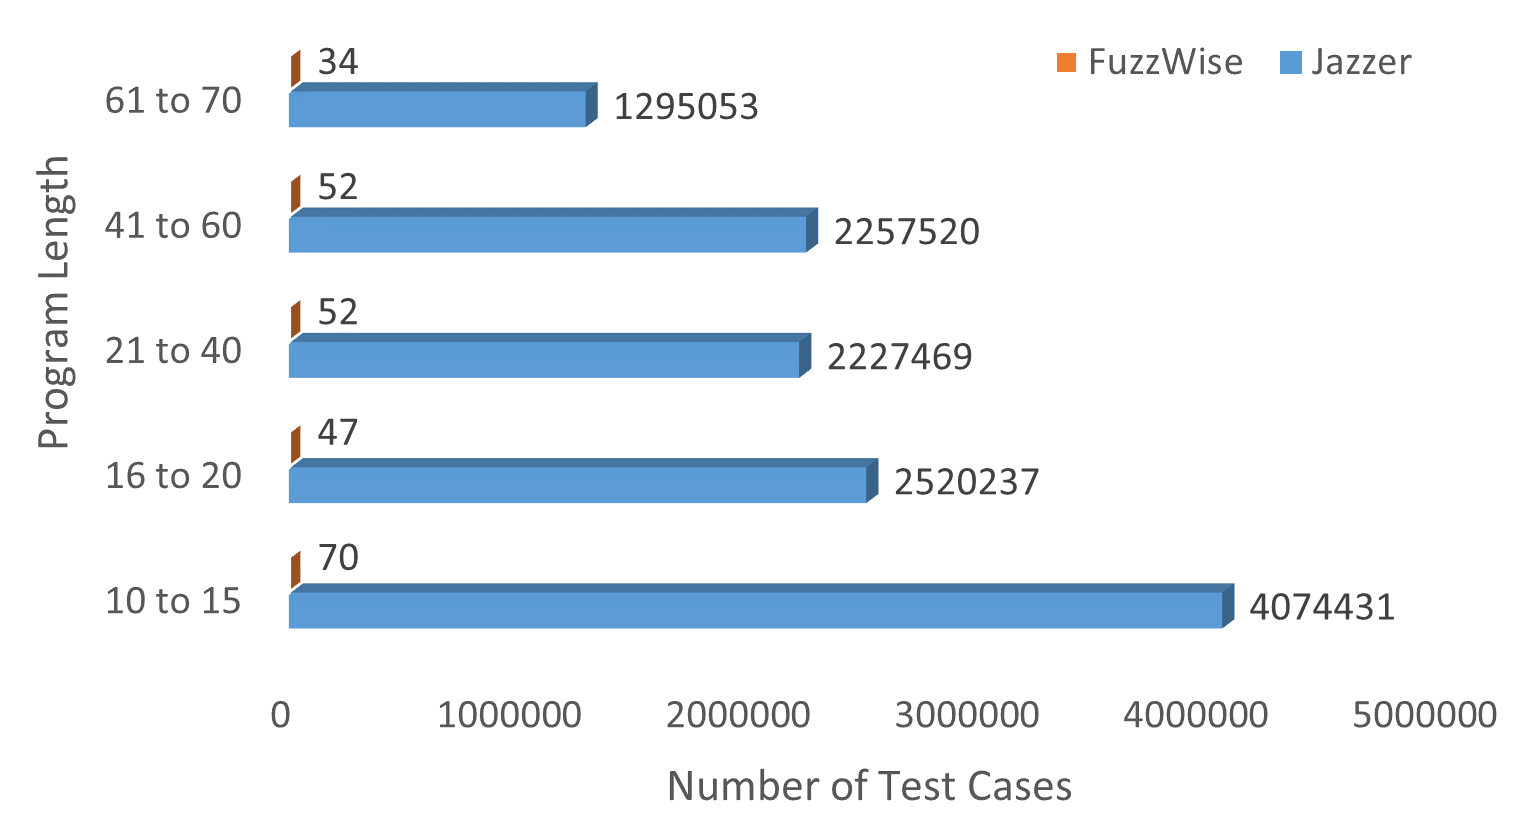
\includegraphics[width=3in]{RQ1b_Discarded Test Cases.png}
\vspace{-20pt}
\caption{Comparison on Test Case Execution and Dismissal}
\label{fig:rq1-agt-aet-adt-graph}
\end{center}
\end{wrapfigure}

Fig.~\ref{fig:rq1-agt-aet-adt-graph} provides a visual comparison
between {\tool} and Jazzer regarding the number of test cases that
were wasted. In the case of Jazzer, these include the test cases
generated through mutations and executed but did not detect any
runtime errors, nor were they included as test seeds for subsequent
test generation cycles. This corresponds to the wasted resources in
the execution of those wasted test cases.  For {\tool}, we counted
towards this metric the generated test cases that were not included in
the final test suite, as well as those that were executed but did not
reveal any runtime errors. As depicted in
Fig.~\ref{fig:rq1-agt-aet-adt-graph}, Jazzer wasted a significantly
higher number of test cases compared to {\tool} across various code
length ranges. For example, for code snippets with 10--15 lines,
Jazzer discards/wastes an average of 4,074,431 test cases, while
{\tool} discards only {\bf 305} test cases. This trend
continues as code length increases, with Jazzer consistently
discarding a substantial number of test cases, whereas {\tool}
discards fewer or none, indicating the higher quality of its test case
generation. This also implies that {\tool} saves a large amount of
execution resources.

It is evident that as all the metrics for both fuzzers consistently decrease (Table~\ref{tab:rq1coverageeval} and Fig.~\ref{fig:rq1-agt-aet-adt-graph}). This trend is attributed to the increased time required to execute and predict code coverage for longer code lengths.

%As seen, regarding the number of test cases generated, {\tool}
%generated a signficantly smaller number of test cases: approximately
%0.0065\% of the number of test cases generated by Jazzer for a
%program, yet it successfully detected a higher number of unique
%runtime exceptions. 

%Furthermore, in terms of the number of test cases generated (refer to Figure 6), {\tool} generated approximately 0.0065\% of the number of test cases generated by Jazzer for a program, yet it successfully raised a higher number of unique runtime exceptions. This can be attributed to the controlled and less random nature of the test case mutations generated by {\tool} compared to Jazzer.

%Regarding the generated test cases that were actually executed, due to
%its design, Jazzer executed all of the generated ones (including the
%duplicate ones), while {\tool} executed an average of 235 out of 315
%generated test cases. For each program, Jazzer on average executed
%{\bf XX} test cases, while {\tool} executed only {\bf XX} test cases.
%Coupled with Fig.\ref{fig:rq1-runtime-detection}, {\tool} is more
%efficiently in runtime error detection than the baseline. On average,
%{\tool} executed {\bf XX} generated test cases to detect a runtime
%error, while Jazzer executed {\bf XX} test cases for an exception.

%Tien: discarded test cases
%Fig.~\ref{fig:rq1-agt-aet-adt-graph} visually displays the comparison
%between {\tool} and Jazzer regarding the numbers of test cases that
%were `disregarded'. For Jazzer, those are the test cases that were
%generated through mutations and executed, but did not detect any
%runtime errors nor were put back as the test seeds for the next cycles
%of test generation.  For {\tool}, we counted toward it the generated
%test cases that were generated, but not included in the final test
%suite and the ones that were executed but did not reveal any runtime
%errors. As seen in Fig.~\ref{fig:rq1-agt-aet-adt-graph}, Jazzer
%discards a significantly higher number of test cases compared to
%{\tool} across various code length ranges. For instance, for code snippets
%with 10--15 lines, Jazzer discards an average of 4,679,532
%test cases, whereas {\tool} discards only 305 test cases. As code
%length increases, Jazzer continues to discard a substantial number of
%test cases, whereas {\tool} discards fewer or none, indicating the
%higher quality of its test case generation.

%From Table~\ref{fig:rq1-agt-aet-adt-table} and
%Fig.~\ref{fig:rq1-agt-aet-adt-graph}, it is noteworthy that as the
%average code length increases, the metrics AGT (Average Generated Test
%cases), AET (Average Executed Test cases), and AGT (Average Discarded
%Test Cases) for both fuzzers consistently decrease due to the
%increased time required to execute and predict code coverage for
%longer code lengths.

%Moreover, when comparing the number of discarded test cases due to ineffectiveness or duplication (refer to Figure 7), Jazzer discards a significantly higher number of test cases compared to {\tool} across various code length ranges. For instance, for code lengths of 10 to 15 lines, Jazzer discards an average of 4,679,532 test cases, whereas {\tool} discards only 305 test cases. As code length increases, Jazzer continues to discard a substantial number of test cases, whereas {\tool} discards fewer or none, indicating the higher quality of its test case mutations, as seen in Figure 6.

%Regarding test case execution, Jazzer executed all generated test cases regardless of duplicate instances, whereas {\tool} executed an average of 235 out of 315 test cases generated.

%This difference arises because {\tool} removes duplicate test cases before execution to enhance efficiency.

%Tien: talk about the ratio of executed test cases over the detected exceptions










